\documentclass[aspectratio=169]{beamer}

\usepackage{fontawesome}
\usepackage{graphicx}
\usepackage{minted}
\usepackage{tikz}

\newcommand{\megatext}[1]{
  \begin{center}
    \Huge
    #1
  \end{center}
}



\title{An experiment in concurrent CSV processing}
\subtitle{When are big data tools really necessary?}
\author{Jonathan E. Magen / \faicon{twitter} @yonkeltron}
\date{Compiled \today}


\begin{document}
\frame{\titlepage}

\begin{frame}{Who is this guy?}
  \begin{itemize}
  \item Computer Scientist
  \item Loves computers
  \item Fascinated by concurrency
  \item On the Big Data team at Cigna (not representing the company)
  \end{itemize}
\end{frame}


\begin{frame}
  \megatext{Big data}
\end{frame}

\begin{frame}
  \begin{figure}
    \includegraphics[keepaspectratio,scale=2]{images/file-icon-csv.pdf}
  \end{figure}
\end{frame}

\begin{frame}
  \megatext{When do you bring in the heavy stuff?}
\end{frame}

\begin{frame}{The experiment}
  \begin{block}{Hypothesis}
    A concurrent, multi-threaded approach to CSV processing will yield better performance and efficiency than a synchronous, single-threaded attempt.
  \end{block}

  \begin{block}{Tools employed}
    \begin{description}
    \item[Ruby] to generate fake data and code
    \item[Scala] for processing data
    \item[Awk] for establishing benchmarks
    \end{description}
  \end{block}
\end{frame}


\begin{frame}{Actual work done}
  \megatext{\texttt{"a,b,c" -> "xax,xbx,xcx"}}
\end{frame}


\begin{frame}[fragile]{Actual work done}
  \inputminted{scala}{snippets/process.scala}

  \begin{itemize}
    \item Pre-splitting the row string
    \item 2 collection traversals
    \item $2*n$ string operations
    \item Building a new row string
  \end{itemize}
\end{frame}


\begin{frame}[fragile]{Awk as baseline}
  \begin{minted}{text}
==> awk
256.21s user 3.41s system 99% cpu 4:20.29 total

==> gawk
102.99s user 2.75s system 99% cpu 1:46.14 total
  \end{minted}
\end{frame}


\begin{frame}
  \megatext{Threads are terrible.}
\end{frame}


\begin{frame}
  \megatext{Actors are pretty good.}
\end{frame}


\begin{frame}{Actors}

  Actors are the primitive, fundamental unit of computation.

  \begin{itemize}
  \item Actors need to have three abilities:
    \begin{itemize}
    \item Processing --- Do things
    \item Storage --- Remember things
    \item Communication --- Talk
    \end{itemize}

  \item Actors have addresses (like capabilites, not the same as identity).

  \item Actor axioms: When an actor receives a message, what can it do?
    \begin{itemize}
    \item Create more actors.
    \item Send messages (requires actor addresses).
    \item Designate what happens with next message (state!).
    \end{itemize}
  \end{itemize}
\end{frame}

\begin{frame}{Actor communication}
  \begin{figure}
    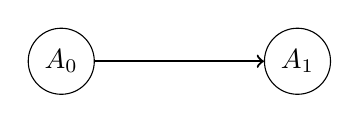
\begin{tikzpicture}
      \node[draw, circle] (one) at (0,0) { $A_0$ };
      \node[draw, circle] (two) at (3,0) { $A_1$ };

      \draw[->, thick] (one) -- (two);
    \end{tikzpicture}
  \end{figure}

  \begin{itemize}
  \item Messages delivered at most once.
  \item Actors have FIFO mailboxes.
  \item Conceptually: Actors process one message at a time.
  \item No channels! No overhead! A channel would be another actor.
  \end{itemize}
\end{frame}


\begin{frame}
  \megatext{Actors in Scala?}
\end{frame}


\begin{frame}
  \begin{figure}
    \includegraphics[keepaspectratio,scale=0.7]{images/Akka_toolkit_logo.pdf}
  \end{figure}
\end{frame}


\begin{frame}
  \begin{columns}[c]
    \begin{column}{0.5\textwidth}
      \begin{itemize}
      \item Futures (now in \texttt{scala.concurrent})
      \item Actors
      \item Streams
      \end{itemize}
    \end{column}

    \begin{column}{0.5\textwidth}
      \begin{figure}
        \includegraphics[keepaspectratio,scale=0.3]{images/Akka_toolkit_logo.pdf}
      \end{figure}
    \end{column}
  \end{columns}
\end{frame}


\begin{frame}[fragile]{Akka Actors}
  \inputminted{scala}{snippets/actor.scala}
\end{frame}

%% \begin{frame}[fragile]{Akka Actors}
%%   \inputminted{scala}{snippets/actors.scala}
%% \end{frame}

\begin{frame}[fragile]{Akka Streams}
  \inputminted{scala}{snippets/streams.scala}
\end{frame}

\begin{frame}[fragile]{Scala Parallel Collections}
  \inputminted{scala}{snippets/pcoll.scala}
\end{frame}

\begin{frame}
  \megatext{Demo}

  \begin{itemize}
  \item Run different Scala strategies
    \begin{itemize}
    \item Synchronous
    \item Actors
    \item Streams
    \item Parallel collections
    \end{itemize}
  \item Monitor memory and CPU performance using VisualVM
  \end{itemize}
\end{frame}

\begin{frame}[fragile]{Results}
  \begin{minted}{text}
==> Synchronous
 96.31s user 17.95s system 101% cpu 1:52.27 total

==> Akka Actors
410.06s user 58.95s system 464% cpu 1:41.00 total

==> Akka Streams
156.59s user 76.67s system 188% cpu 2:03.98 total

==> Scala Parallel collections
165.46s user 46.78s system 297% cpu 1:11.30 total
  \end{minted}
\end{frame}

\begin{frame}
  \megatext{End. Thank you.}
  \Large
  \centering
  Jonathan E. Magen / \faicon{twitter} @yonkeltron
\end{frame}
\end{document}
